\documentclass[border=5pt]{standalone}
\usepackage{xcolor}
\usepackage{tikz}
\usepackage{adjustbox}
\usetikzlibrary{shapes.geometric, arrows, positioning, fit, backgrounds}

\definecolor{clBlue}   {RGB}{41,  98, 175}
\definecolor{clPurple} {RGB}{103,  58, 183}
\definecolor{clRed}    {RGB}{198,  40,  40}
\definecolor{clOrange} {RGB}{230, 119,   0}
\definecolor{clTeal}   {RGB}{  0, 121, 107}
\definecolor{clGreen}  {RGB}{ 46, 125,  50}
\definecolor{clGray}   {RGB}{ 80,  80,  80}
\definecolor{clGold}   {RGB}{175, 141,   0}

\begin{document}
\begin{adjustbox}{max width=\linewidth}
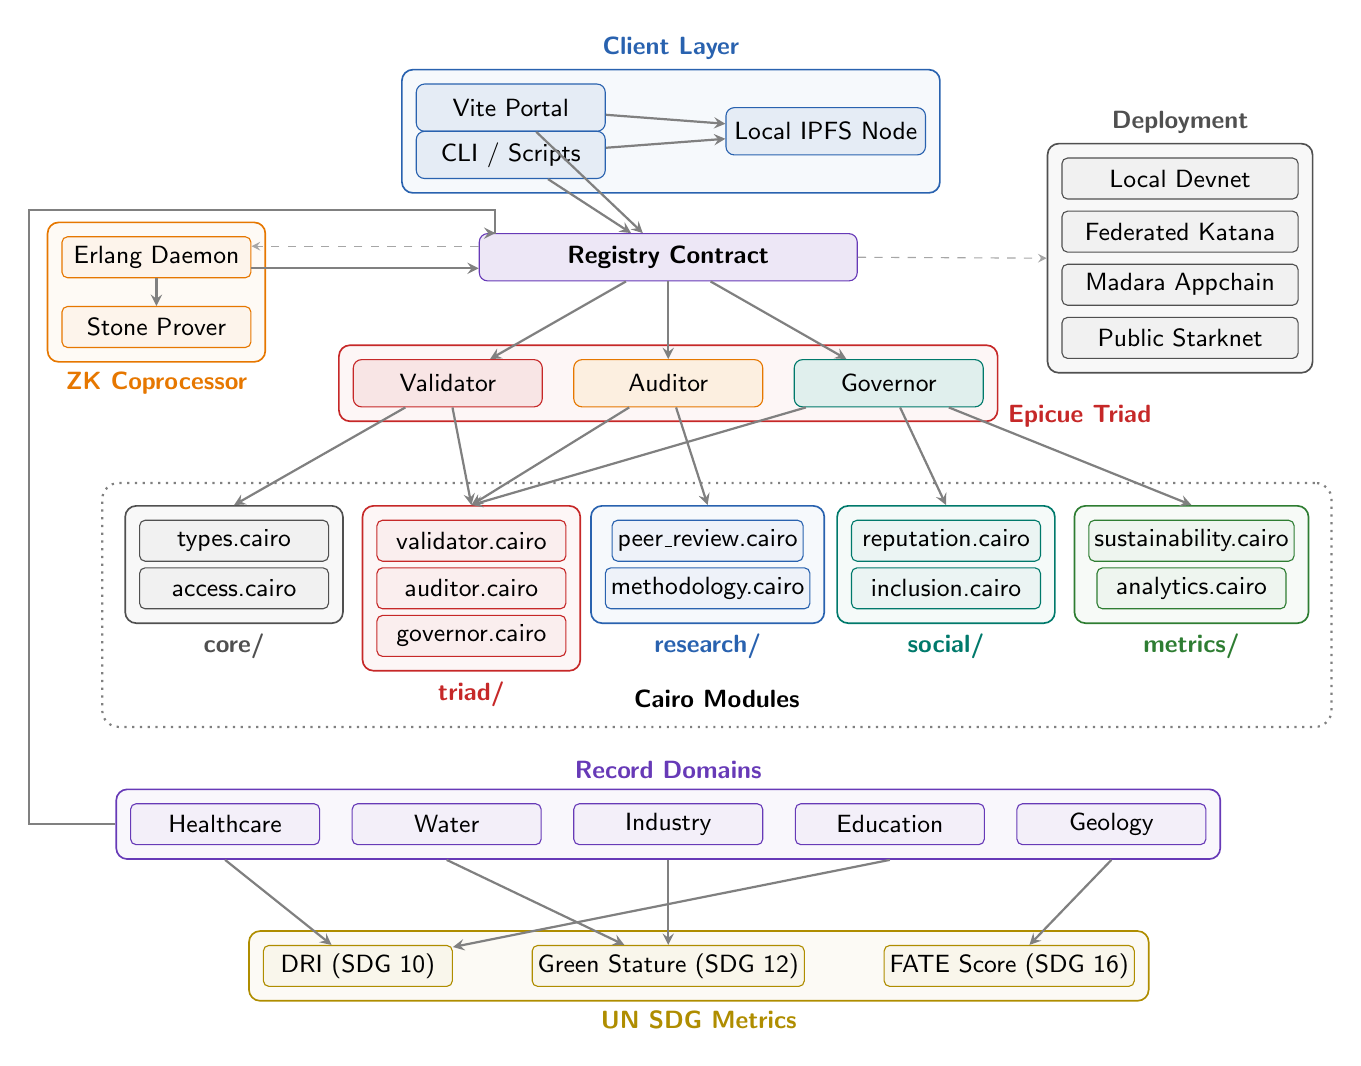
\begin{tikzpicture}[
    font=\small\sffamily,
    transform shape,
    >={stealth},
    layer/.style   = {rectangle, rounded corners=3pt, draw=#1, fill=#1!12!white, minimum width=2.4cm, minimum height=0.6cm, text centered, inner sep=3pt},
    mod/.style     = {rectangle, rounded corners=2pt, draw=#1, fill=#1!8!white, minimum width=2.4cm, minimum height=0.52cm, text centered, font=\small\sffamily, inner sep=2pt},
    grpbox/.style  = {rectangle, rounded corners=4pt, draw=#1, fill=#1!4!white, inner sep=5pt, line width=0.6pt},
    arr/.style     = {->, thick, draw=black!50},
    darr/.style    = {->, dashed, draw=black!35},
    lbl/.style     = {font=\small\bfseries\sffamily},
]

%% ── Row 0 ──────────────────────────────────────────────────────────────────
\node[layer=clBlue] (portal) at (-2.0,0.3) {Vite Portal};
\node[layer=clBlue] (cli)    at (-2.0,-0.3) {CLI / Scripts};
\node[layer=clBlue] (ipfs)   at (2.0,0) {Local IPFS Node};
\begin{pgfonlayer}{background}
  \node[grpbox=clBlue, fit=(portal)(cli)(ipfs), label={[lbl,text=clBlue]above:Client Layer}] (clients) {};
\end{pgfonlayer}

%% ── Row 1 ──────────────────────────────────────────────────────────────────
\node[layer=clPurple, minimum width=4.8cm] (registry) at (0,-1.6) {\textbf{Registry Contract}};

%% ── Row 2 ──────────────────────────────────────────────────────────────────
\node[layer=clRed]    (validator) at (-2.8,-3.2) {Validator};
\node[layer=clOrange] (auditor)   at ( 0,  -3.2) {Auditor};
\node[layer=clTeal]   (governor)  at ( 2.8,-3.2) {Governor};
\begin{pgfonlayer}{background}
  \node[grpbox=clRed, fit=(validator)(auditor)(governor), label={[lbl,text=clRed,yshift=-12pt]right:Epicue Triad}] (triad) {};
\end{pgfonlayer}

%% ── Row 3 ──────────────────────────────────────────────────────────────────
\node[mod=clBlue] (rpr) at (0.5,-5.2) {peer\_review.cairo};
\node[mod=clBlue, below=2pt of rpr] (rmeth) {methodology.cairo};
\begin{pgfonlayer}{background}
  \node[grpbox=clBlue, fit=(rpr)(rmeth), label={[lbl,text=clBlue]below:research/}] (resmod) {};
\end{pgfonlayer}

\node[mod=clRed] (tvalid) at (-2.5,-5.2) {validator.cairo};
\node[mod=clRed, below=2pt of tvalid] (taudit) {auditor.cairo};
\node[mod=clRed, below=2pt of taudit] (tgovern) {governor.cairo};
\begin{pgfonlayer}{background}
  \node[grpbox=clRed, fit=(tvalid)(taudit)(tgovern), label={[lbl,text=clRed]below:triad/}] (triadmod) {};
\end{pgfonlayer}

\node[mod=clGray, left=0.6cm of tvalid] (types) {types.cairo};
\node[mod=clGray, below=2pt of types] (access) {access.cairo};
\begin{pgfonlayer}{background}
  \node[grpbox=clGray, fit=(types)(access), label={[lbl,text=clGray]below:core/}] (coremod) {};
\end{pgfonlayer}

\node[mod=clTeal, right=0.6cm of rpr] (srep) {reputation.cairo};
\node[mod=clTeal, below=2pt of srep] (sincl) {inclusion.cairo};
\begin{pgfonlayer}{background}
  \node[grpbox=clTeal, fit=(srep)(sincl), label={[lbl,text=clTeal]below:social/}] (socmod) {};
\end{pgfonlayer}

\node[mod=clGreen, right=0.6cm of srep] (msust) {sustainability.cairo};
\node[mod=clGreen, below=2pt of msust] (manal) {analytics.cairo};
\begin{pgfonlayer}{background}
  \node[grpbox=clGreen, fit=(msust)(manal), label={[lbl,text=clGreen]below:metrics/}] (metmod) {};
\end{pgfonlayer}

\coordinate (cairomod_bottom) at ([yshift=-12pt]triadmod.south);
\begin{pgfonlayer}{background}
  \node[draw=black!50, dotted, line width=0.8pt, rounded corners=6pt, inner sep=8pt, fit=(coremod)(triadmod)(resmod)(socmod)(metmod)(cairomod_bottom)] (cairomods) {};
\end{pgfonlayer}

%% ── Row 4 ──────────────────────────────────────────────────────────────────
\node[mod=clPurple] (dind) at (0, -8.8) {Industry};
\node[mod=clPurple, left=0.4cm of dind]  (dwat) {Water};
\node[mod=clPurple, left=0.4cm of dwat]  (dhc)  {Healthcare};
\node[mod=clPurple, right=0.4cm of dind] (dedu) {Education};
\node[mod=clPurple, right=0.4cm of dedu] (dgeo) {Geology};
\begin{pgfonlayer}{background}
  \node[grpbox=clPurple, fit=(dhc)(dwat)(dind)(dedu)(dgeo), label={[lbl,text=clPurple]above:Record Domains}] (domains) {};
\end{pgfonlayer}

%% ── Row 5 ──────────────────────────────────────────────────────────────────
\node[mod=clGold] (sdggsi)  at (0, -10.6) {Green Stature (SDG 12)};
\node[mod=clGold, left=1.0cm of sdggsi]  (sdgdri)  {DRI (SDG 10)};
\node[mod=clGold, right=1.0cm of sdggsi] (sdgfate) {FATE Score (SDG 16)};
\begin{pgfonlayer}{background}
  \node[grpbox=clGold, fit=(sdgdri)(sdggsi)(sdgfate), label={[lbl,text=clGold]below:UN SDG Metrics}] (sdgs) {};
\end{pgfonlayer}

%% ── ZK Coprocessor ─────────────────────────────────────────────────────────
\node[mod=clOrange] (daemon) at (-6.5,-1.6) {Erlang Daemon};
\node[mod=clOrange, below=10pt of daemon] (prover) {Stone Prover};
\begin{pgfonlayer}{background}
  \node[grpbox=clOrange, fit=(daemon)(prover), label={[lbl,text=clOrange]below:ZK Coprocessor}] (coproc) {};
\end{pgfonlayer}

%% ── Deployment ─────────────────────────────────────────────────────────────
\node[mod=clGray, minimum width=3.0cm] (devnet)     at (6.5,-0.6) {Local Devnet};
\node[mod=clGray, minimum width=3.0cm, below=4pt of devnet] (fedkatana) {Federated Katana};
\node[mod=clGray, minimum width=3.0cm, below=4pt of fedkatana] (madara) {Madara Appchain};
\node[mod=clGray, minimum width=3.0cm, below=4pt of madara] (sepolia) {Public Starknet};
\begin{pgfonlayer}{background}
  \node[grpbox=clGray, fit=(devnet)(sepolia), label={[lbl,text=clGray]above:Deployment}] (deploy) {};
\end{pgfonlayer}

%% ── Edges ──────────────────────────────────────────────────────────────────
\draw[arr] (portal) -- (ipfs);
\draw[arr] (cli) -- (ipfs);
\draw[arr] (portal) -- (registry);
\draw[arr] (cli) -- (registry);
\draw[arr] (registry) -- (validator);
\draw[arr] (registry) -- (auditor);
\draw[arr] (registry) -- (governor);
\draw[arr] (validator) -- (coremod.north);
\draw[arr] (validator) -- (triadmod.north);
\draw[arr] (auditor) -- (resmod.north);
\draw[arr] (auditor) -- (triadmod.north);
\draw[arr] (governor) -- (socmod.north);
\draw[arr] (governor) -- (metmod.north);
\draw[arr] (governor) -- (triadmod.north);

\draw[arr] (domains.west) -- ++(-1.1,0) |- (-2.2,-1.0) |- ([xshift=6pt]registry.north west);
\draw[arr] (domains.south -| dhc) -- (sdgdri);
\draw[arr] (domains.south -| dedu) -- (sdgdri);
\draw[arr] (domains.south -| dwat) -- (sdggsi);
\draw[arr] (domains.south -| dind) -- (sdggsi);
\draw[arr] (domains.south -| dgeo) -- (sdgfate);
\draw[darr] (registry.east) -- (deploy.west);

\draw[darr] ([yshift=4pt]registry.west) -- ([yshift=4pt]daemon.east);
\draw[arr] ([yshift=-4pt]daemon.east) -- ([yshift=-4pt]registry.west);
\draw[arr] (daemon) -- (prover);

\node[lbl, text=black, anchor=south, yshift=4pt] at (cairomods.south) {Cairo Modules};

\end{tikzpicture}
\end{adjustbox}
\end{document}
